
This chapter presents some aspects of the graphical interface of \Eva{}. More
information can be found in the Frama-C blog, under the keyword
\texttt{tutorial}.
Some examples shown in this section are taken from the Monocypher tutorial,
presented in the blog.
% The source code used in this tutorial is the version 0.3 of
% \href{http://loup-vaillant.fr/projects/monocypher/}{Monocypher}, a
% C99-conformant crytographic library that also includes a nice test
% suite\footnote{The archive for version 0.3 is available at
% \href{http://loup-vaillant.fr/projects/monocypher/monocypher-0.3.tar.gz}.}.


\paragraph{A caveat.}

As a general recommendation,
  \textbf{do not} start your analyses within the GUI.
  Use the command-line. You should
  consider Frama-C/\Eva{} as a command-line tool with a viewer (the GUI).
  The Frama-C GUI is not an IDE (e.g.~you cannot edit code with it), and
  \Eva{} does not use the GUI for anything else other than rendering its
  results. It is recommended to run the value analysis using the command line,
  and then saving the result to a Frama-C save file
  (see Section~\ref{three-step}).

\section{A general view of the GUI}

After running the value analysis and saving your results,
it is a good time to check what the result looks like, using the GUI:

\begin{verbatim}
frama-c-gui -load value.sav
\end{verbatim}

In the screenshot of Figure~\ref{fig:gui-eva},
we indicate some parts of the GUI that are
useful when inspecting \Eva{} results (besides the source view). We also
indicate some parts that are never (or rarely) used with \Eva{}.

\begin{figure}[hbt]
\centering
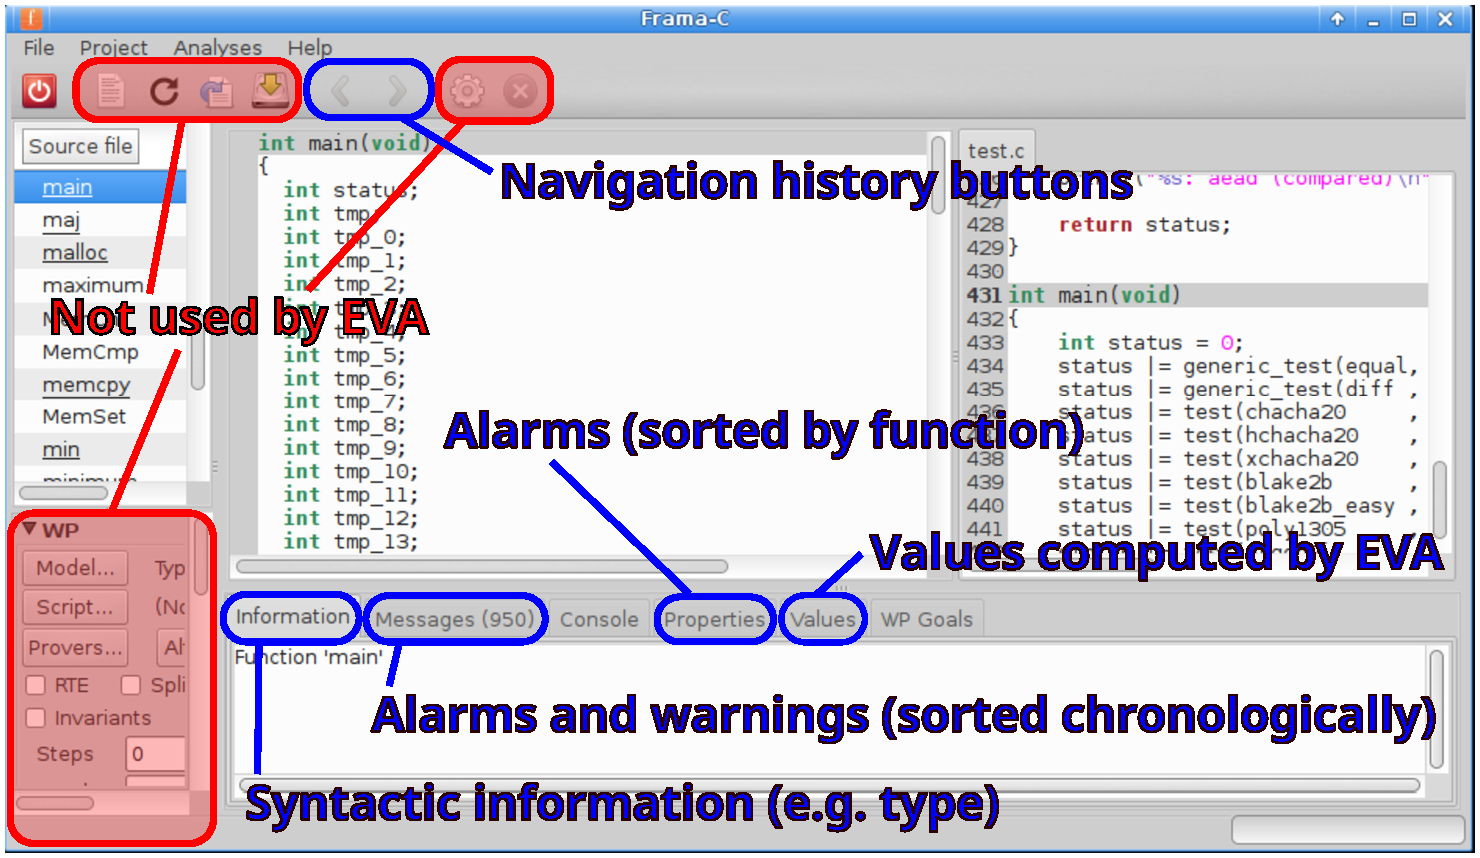
\includegraphics[width=\textwidth]{gui-images/gui1-annotated.pdf}
\caption{Frama-C GUI for \Eva{}}
\label{fig:gui-eva}
\end{figure}

Note that the Properties tab (between Console and Values) is not updated
automatically: you need to click on the \emph{Refresh} button before it
outputs anything, and after changing filters.

Like many GUI-integrated plug-ins, \Eva{} also has a side panel
that is displayed below the globals list, on the lower left corner of the GUI.
This panel can be folded/unfolded using the arrow button on the left,
and when unfolded (Figure~\ref{fig:gui-side-panel}) it displays some controls.
The {\em Run} button runs (or re-runs) the
analysis, using the specified slevel and with the specified main function.
This is useful only for small examples and rarely used in practice.
Also, notice that emitted warnings are persistent in the GUI, so even if a new
run of the value analysis (e.g.~with higher slevel) produces less alarms, the
previous warnings will still be displayed in the {\em Messages} panel.

The checkbox {\em Show list of red alarms} shows or hides the
{\em Red alarms} panel, described in Section~\ref{red-alarms}.

\begin{figure}
\centering
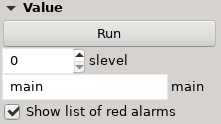
\includegraphics[scale=0.7]{gui-images/gui-side-panel.png}
\caption{GUI side panel for \Eva{}}
\label{fig:gui-side-panel}
\end{figure}


\section{Detecting and understanding non-termination}
\label{sec:non-termination-gui}

Assume that the log of your analysis contains the \texttt{NON\
  TERMINATING\ FUNCTION} message for the \texttt{main} function.
We know that
at some point in the program we will have red statements in the GUI,
which indicate unreachable code.

By scrolling down from the \texttt{main} function, we reach the
non-terminating statement, which in our example is a call to
\texttt{test\_x25519} (Figure~\ref{fig:gui-unreachable}).

\begin{figure}[hbt]
\centering
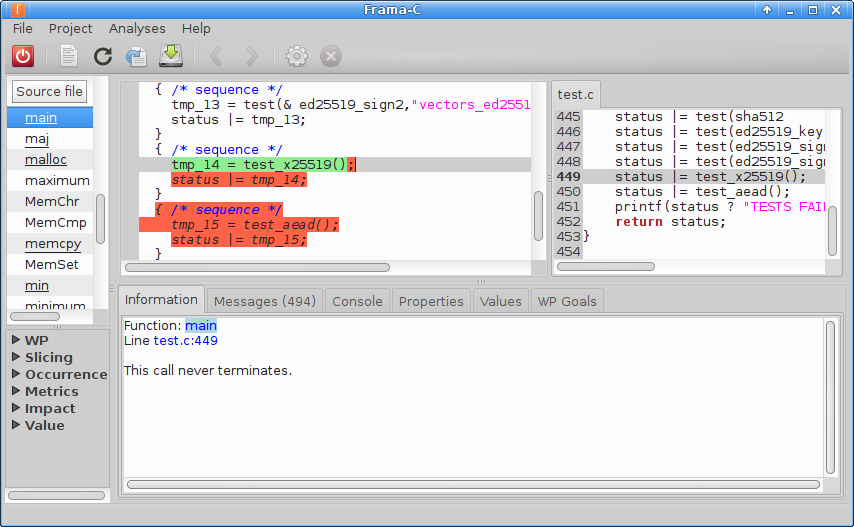
\includegraphics[width=\textwidth]{gui-images/gui2.png}
\caption{Unreachable code in the Frama-C GUI}
\label{fig:gui-unreachable}
\end{figure}

Note the red semicolon at the end of the statement, and the fact that
the statements that follow it are also red. If we click on the statement, the
\emph{Information} panel says that \emph{This call never terminates}.

You can right-click on the function and \emph{Go to the definition of
\texttt{test\_x25519}}, and you will find the same thing inside, this time a call
to \texttt{crypto\_x25519\_public\_key}, and so on, until you reach
\texttt{fe\_tobytes}, which is slightly different: it contains a
\texttt{for} loop (defined via a macro \texttt{FOR}), after which all
statements are red, but the loop itself is not an infinite loop: it
simply iterates \texttt{i} from 0 to 5. How can this be non-terminating?

The answer, albeit non-intuitive, is simple: there is one statement
inside the loop which is non-terminating, but \emph{not} during the
first iteration of the loop. Because the GUI colors are related to the
consolidated result of all callstacks (i.e., if there is at least one
path which reaches a statement, it is marked as reachable), it cannot
show precisely which callstack led to the non-termination.

% To better
% understand what happens here, we will use the \emph{Nonterm} plug-in.
% TODO

\section{Values Panel}\label{values-panel}

The Values panel, depicted in Figure~\ref{fig:values-panel}, is arguably
the most powerful inspection tool for the \Eva{} plug-in in the Frama-C GUI.

\begin{figure}[hbtp]
\centering
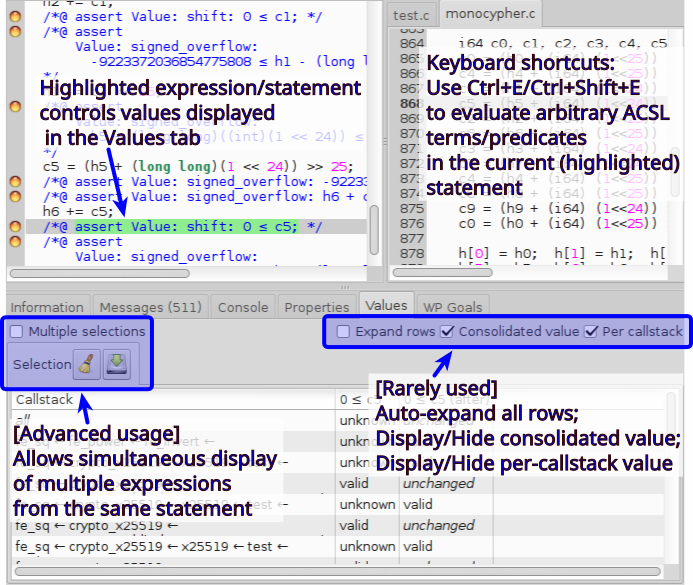
\includegraphics[width=\textwidth]{gui-images/gui-values-annotated.png}
\caption{Values panel}
\label{fig:values-panel}
\end{figure}

The values displayed in this panel are related to the green highlighted
zone in the Cil source. This zone can be a statement, an expression,
an ACSL annotation, etc. Composite expressions can be selected by clicking
on or near their operators. Each kind of selected expression has a set
of associated context menus. For instance, an expression corresponding
to a variable contains a \emph{Go to definition} context menu when
right-clicked on.

The Ctrl+E shortcut is equivalent to highlighting a statement, then
right-clicking \emph{Evaluate ACSL term}. This opens a dialog
(Figure~\ref{fig:eval-acsl}) where you can enter an arbitrary ACSL
term. Its value will be evaluated in the current statement and
displayed in the \emph{Values} panel.

\begin{figure}[!hbtp]
\centering
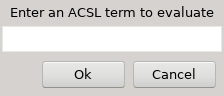
\includegraphics[scale=0.7]{gui-images/eval-acsl.png}
\caption{Evaluate ACSL term dialog, accessible via a context menu or
  by pressing Ctrl+E.}
\label{fig:eval-acsl}
\end{figure}

The Ctrl+Shift+E shortcut is slightly more powerful: it also evaluates
\emph{predicates}, such as \texttt{\textbackslash{}valid(p)}.
This command is not available from any menu.

The \emph{Multiple selections} checkbox allows adding several
expressions to be compared side-by-side. When checked, highlighting an
expression in the same statement adds a column with its value. Note that
highlighting a different statement results in resetting all columns.

The three checkboxes to the right are seldom used (their default values
are fine most of the time): \emph{Expand rows}
simply expands all callstacks (but generates visual clutter);
\emph{Consolidated value} displays the row \emph{all} (union of all
callstacks); and \emph{Per callstack} displays a row for each separate
callstack.

The callstacks display has several contextual menus that can be accessed
via right-clicks (Figure~\ref{fig:callstacks}).

\begin{figure}[hbtp]
\centering
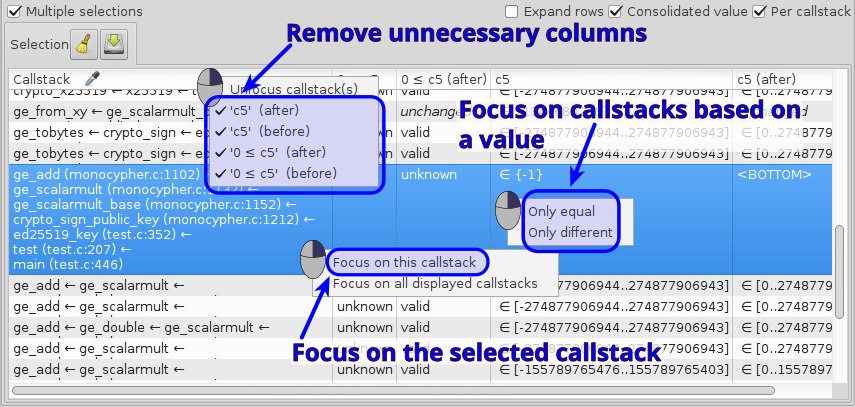
\includegraphics[width=\textwidth]{gui-images/gui-callstacks-annotated.png}
\caption{Callstacks display}
\label{fig:callstacks}
\end{figure}

Let us start from the bottom: right-clicking on a callstack shows a
popup menu that allows you to \emph{focus} on a given callstack. This
focus modifies the display in the Cil code viewer: reachability will
only be displayed for the focused callstack(s). We will come back to
that later.

Right-clicking on a cell containing a value allows filtering on all
callstacks for which the expression has the same value. This is often
used, for instance, to focus on all callstacks in which a predicate
evaluates to \emph{invalid} or \emph{unknown}.

Finally, clicking on the column headers allows filtering columns.

Note that the Callstacks column header displays a pipette icon when a
filter is being applied, to remind you that other callstacks exist.

\subsection{Filtering non-terminating callstacks}
\label{filtering-non-terminating-callstacks}

In our code, despite the existence of 40 callstacks, only one of them is
non-terminating. If you highlight the \texttt{0\ $\le$\ c5} expression
before statement \texttt{h5\ -=\ c5\ \textless{}\textless{}\ 25}, you
will see that only a single callstack displays \emph{invalid} in the
column \texttt{0\ $\le$\ c5}. Focus on this callstack using the popup menu,
then highlight expression \texttt{c5} in the Cil code. You will obtain
the result displayed in Figure~\ref{fig:non-term-callstack}.

\begin{figure}[hbt]
\centering
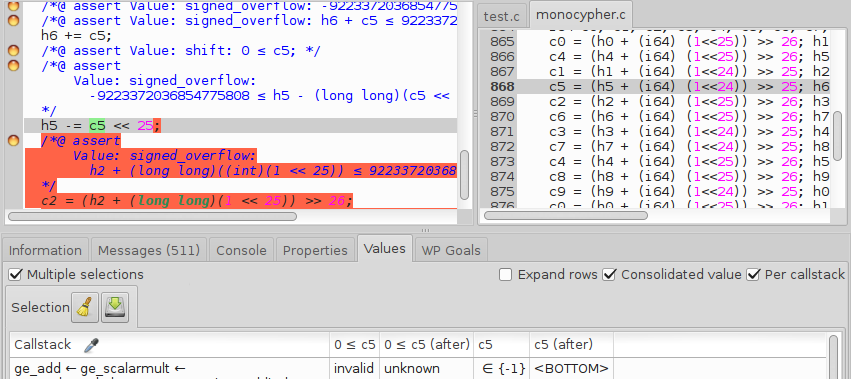
\includegraphics[width=\textwidth]{gui-images/gui5.png}
\caption{Focused on a non-terminating callstack}
\label{fig:non-term-callstack}
\end{figure}

As you can see, the GUI now displays the statements following
\texttt{h5\ -=\ c5\ \textless{}\textless{}\ 25} in red, indicating thay
they are unreachable in the currently focused callstacks. The exact
value that caused this is shown in column \texttt{c5}: \texttt{-1}. The
C standard considers the left-shift of a negative number as undefined
behavior. Because \texttt{-1} is the only possible value in this
callstack, the reduction caused by the alarm leads to a post-state that
is \texttt{\textless{}BOTTOM\textgreater{}}.

\section{Finding origins of alarms and imprecisions via the Studia plug-in}
\label{studia}

The Studia\footnote{The name \emph{Studia} is related to its applicability
to case studies.} plug-in is used to track the origins of values computed by \Eva{}.
For a given lvalue, it highlights all statements that may have written/read
it.

Studia is invoked by right-clicking on a lvalue, selecting the \emph{Studia}
menu, then the \emph{Writes} or \emph{Reads} menu (see Figure~\ref{fig:studia}).
This will highlight all the instructions that may have defined (or read)
the selected lvalue.
\emph{Studia} can also be used on arbitrary lvalues: when called through
the right-click menu with no lvalue selected, \emph{Studia} displays a
dialog box in which an arbitrary lvalue can be typed.

When a lvalue is highlighted, a new column (\emph{Studia}) appears on the
file tree. It shows a check mark next to each function that directly
writes/reads the highlighted lvalue, and an arrow next to each function
that \emph{indirectly} writes/reads the chosen value, that is, the callers of the
functions marked with a check mark.

Each statement writing/reading the chosen value is highlighted in orange in the
Cil code. Different shades of orange are used to distinguish between direct and
indirect accesses.

\begin{figure}[h!]
  \caption{\label{fig:studia}Studia elements in the GUI}
  \centering
    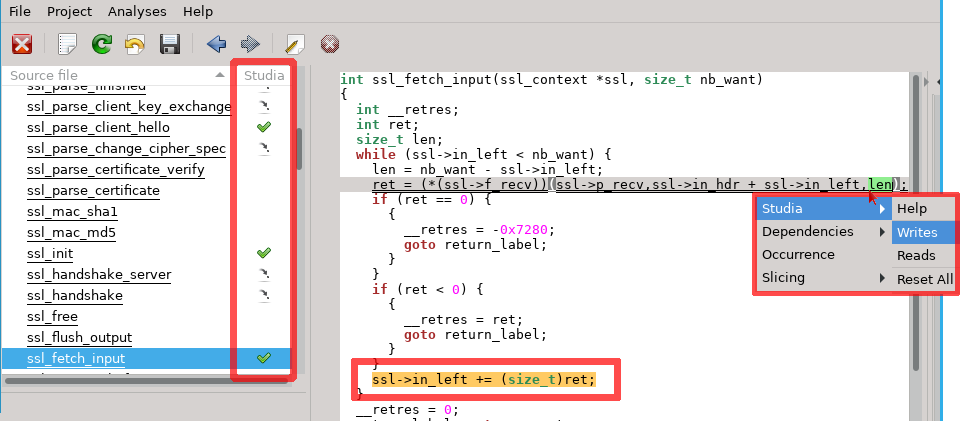
\includegraphics[width=\textwidth]{gui-images/studia}
\end{figure}

Typical usage of Studia consists in: starting the GUI, selecting an alarm
(for instance, a possibly invalid memory access), inspecting the lvalue
that causes the alarm (usually an imprecise value), then using Studia to find
where the lvalue was defined. To find the root cause of a given loss of
precision, it may be necessary to reiterate the process.

\section{Detecting branches abandoned because of red alarms}
\label{red-alarms}

When analyzing code, the value analysis sometimes encounters undefined
behaviors so severe that the analysis cannot proceed afterwards.
This is the case in the code fragment below: no state remains to be
propagated after the addition, because the uninitialized access is guaranteed.

\begin{lstlisting}
int x;
int y = x + 1;
\end{lstlisting}

This example is marked as non-terminating, both in the textual log and in
the GUI.
%
However, things are not always as clear-cut. Replace \lstinline+x+ by
a pointer access, and imagine that only in \emph{some} contexts the memory
location is uninitialized.

\begin{lstlisting}
void f(int *p) {
  if (rand ()) {
    int y = *p + 1;
  }
}

void main() {
  int x = 1, y;
  f(&x);
  f(&y);
}
\end{lstlisting}
In this example, all intructions ``terminate'' in the sense of
Section~\ref{sec:non-termination-gui}. Yet, one branch is cut abruptly
in the analysis of \lstinline+f+.

Even more insidious is a loop where an operation fails only in the last
iterations. In the example below, accessing \lstinline|t[i]| with
\lstinline|i==10| is always invalid, but this is neither reflected
in the Properties panel nor in the Values panel.

\begin{lstlisting}
void main() {
  int i, t[10];
  for (i=0; i<10; i++) {
    t[i] = i;
  }
  int j = 0;
  for (i=0; i<=10; i++) {
    j += t[i];
    if (rand ()) break;
  }
}
\end{lstlisting}

The {\em Red alarms} panel (Figure~\ref{fig:red-alarms-panel}) can be used to
detect such kinds of severe alarms.
The semantics it implements is the following: if in at least \emph{one}
analysis context, the alarm received an Invalid status (the ACSL property
does not hold), then the alarm is present in the panel.
Back to our second example, \lstinline+\initialized(p)+ is false.
The \emph{Nb contexts} column indicates in how many callstacks such an Invalid
status was emitted during the analysis.

\begin{figure}[htbp]
\centering
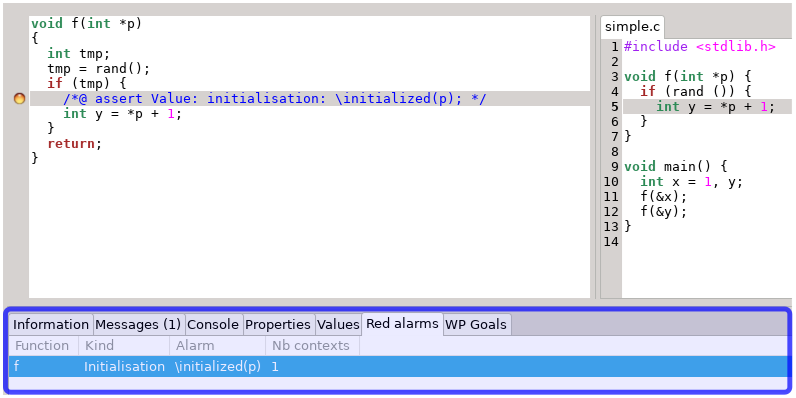
\includegraphics[width=\textwidth]{gui-images/gui-red-alarms-panel.png}
\caption{Red alarms panel}
\label{fig:red-alarms-panel}
\end{figure}

Information on non-terminating branches is also available through
the \emph{Values} panel (Figure~\ref{fig:red-values}). Once you have selected
a property listed in the \emph{Red alarms} panel, a new column appears,
which displays red indicators.
The way to read this information is: ``in this context,
the property evaluated to false at least once''.

\begin{figure}[htbp]
\centering
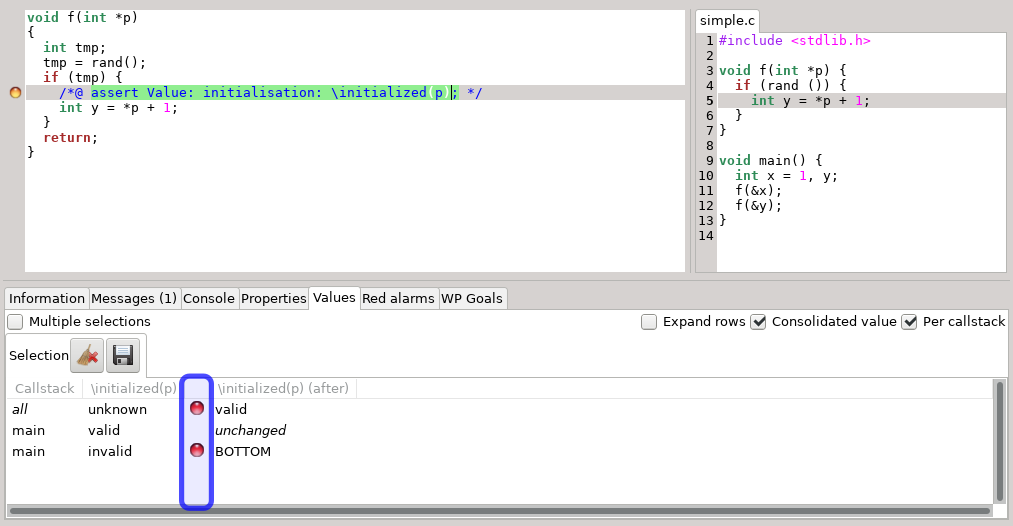
\includegraphics[width=\textwidth]{gui-images/gui-red-values.png}
\caption{Indicators of red alarms in the Values panel}
\label{fig:red-values}
\end{figure}



%% Local Variables:
%% TeX-master: "main.tex"
%% ispell-local-dictionary: "english"
%% End:
